\documentclass[a4paper]{article}

\usepackage{amsmath,amssymb,bm}
\usepackage[british]{babel}
\usepackage{graphicx}
\usepackage{titlesec}
\usepackage{xltxtra}
\usepackage{titling}
\usepackage[font=sf]{caption}
\usepackage{subfig}
\usepackage{siunitx}

\setmainfont[Ligatures=TeX]{PT Serif}
\setsansfont[Ligatures=TeX]{PT Sans}

\usepackage{xpatch}
\xapptocmd\normalsize{
 \abovedisplayskip=15pt
 \abovedisplayshortskip=10pt
 \belowdisplayskip=15pt
 \belowdisplayshortskip=10pt
}{}{}

\captionsetup[subfigure]{font=sf}

\titleformat*{\section}{\Large\bfseries\sffamily}


\pretitle{
	\vspace{-60pt}
  \noindent\rule{\linewidth}{1pt}\vspace{15pt}
	\fontsize{21}{25}\sffamily\bfseries
}

\posttitle{\par\vskip 15pt}

\preauthor{
  \noindent\fontsize{14}{20}\sffamily\noindent
}

\postauthor{
	\vspace{10pt}
  \par\noindent\rule{\linewidth}{1pt}\vspace{15pt}
	\vspace{20pt}
}

% Here we are.

\title{Statistical analysis of super-resolution single particle trajectories}
\author{Matteo Dora \newline\newline \small{\mbox{matteo.dora@polito.it}}}

\date{\today}

\begin{document}
\maketitle

\section{Introduction}

A dataset of single particle trajectories sampled at \SI{125}{ms} was analyzed. The goal was to recover a description of the physical and dynamical properties of the particles (e.g. diffusion, drift field) by means of statistical analysis.

In particular I was interested in studying two features of the drift field: attractors and channels. Attractors (or wells) are regions of the space where the drift field vanishes and the particles can escape only by diffusion. Channels instead are paths along which particles are funneled together and pushed at high speed from one region to another.

The dataset consisted in \SI{\sim 350 000} datapoints belonging to \SI{\sim 20 000} trajectories. The spatial distribution of the datapoints is visible in figure \ref{fig:datapoints}.

\begin{figure}[h]
  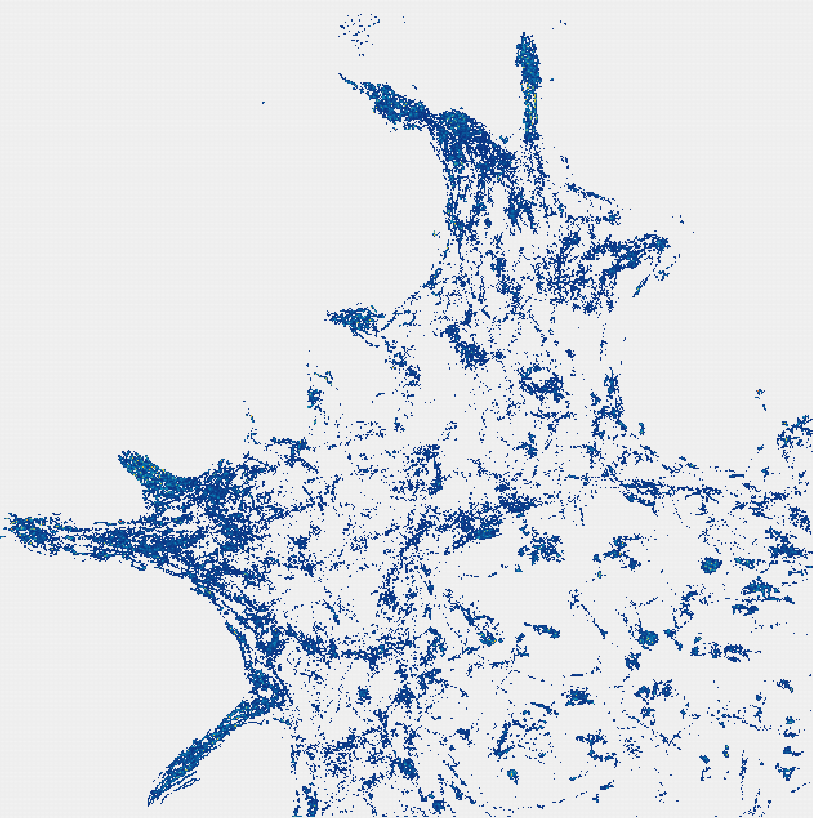
\includegraphics[width=\linewidth]{img/01_datapoints.png}
  \caption{Dataset points at a resolution of \SI{100}{nm}}
  \label{fig:datapoints}
\end{figure}

\section{Physical model}

\subsection{Effective dynamical model}

At the microscopic level the motion of the molecules can be described by the Langevin equation, which in the case of biological processes we are interested in can be considered in its large friction limit (Smoluchowski's equation)
\begin{equation} \label{eq:smoluchowski}
\dot{\bm{x}} = \frac{\bm{F}(\bm{x})}{\gamma} + \sqrt{2D} \dot{\bm{w}}
\end{equation}
where $\bm{F}(\bm{x})$ is the drift force exerted on the particle at position $\bm{x}$, $\gamma$ is the friction coefficient, $D$ is the diffusion coefficient and $\bm{w}(t)$ is a two-dimensional Wiener process. For this microscopic model we expect the diffusion to be due to thermal agitation and we can consider it isotropic.

However, the empirical data have a finite resolution in space and time due to obvious limits of the acquisition device. It is thus not possible to recover the microscopic model, since we miss information about the local behaviour both in space (e.g. the presence of microscopic obstacles) and time (e.g. thermal fluctuations are much faster than the measuring timescale). Yet we can build a coarse-grained model transforming eq. \ref{eq:smoluchowski} into the effective stochastic equation \cite{hoze2012} \cite{hoze2014}
\begin{equation} \label{eq:coarse-grained}
\dot{\bm{x}} = \bm{a}(\bm{x}) + \sqrt{2}\bm{B} \dot{\bm{w}}
\end{equation}
where $\bm{a}(\bm{x})$ is the effective drift field and $\bm{D} \equiv \bm{B}^T\bm{B}$ is the effective diffusion tensor. Note that in this coarse-grained model the diffusion coefficient cannot be considered isotropic because it takes into account the microscopic local features (e.g. obstacles).

\subsection{Reconstructing the drift and diffusion coefficients}

It is possible to reconstruct the effective drift and diffusion tensor of the coarse-grained model of eq. \ref{eq:coarse-grained} from the trajectories increments \cite{hoze2014} \cite{schuss} with
\begin{align}
a^i(\bm{x}) &= \lim_{\Delta t \to 0}\frac{\mathbb{E}\left[x^i(t + \Delta t) - x^i(t) \mid \bm{x}(t) = \bm{x}\right]}{\Delta t} \label{eq:drift}\\[10pt]
2D^{ij}(\bm{x}) &= \lim_{\Delta t \to 0}\frac{\mathbb{E}\left[\left(x^i(t + \Delta t) - x^i(t)\right)\left(x^j(t + \Delta t) - x^j(t)\right) \mid \bm{x}(t) = \bm{x}\right]}{\Delta t} \label{eq:diff}
\end{align}
where the expected value is taken on the trajectories that pass through $\bm{x}$ at time $t$.

We can translate eq. \ref{eq:drift} and \ref{eq:diff} into statistical estimators by grouping the trajectories in a small neighbourhood of $\bm{x}$ and then performing the average. For convenience I chose to divide the space using a grid of identical square bins $S_l(\bm{x})$ characterized by side $l$ and center $\bm{x}$.

It is convenient to define $\Delta \bm{x}_k(t_m) \equiv \bm{x}_k(t_m + \Delta t) - \bm{x}_k(t_m)$, i.e the $m$-th step of the trajectory $k$. The estimators can then be defined as

\begin{align}
\hat{a}^i({\bm{x}}) &= \frac{1}{N} \sum_{\bm{x}_k(t_m) \in S_l(\bm{x})} \frac{\Delta x_k^i(t_m)}{\Delta t} \label{eq:drift-estimator} \\[10pt]
\hat{D}^{ij} &= \frac{1}{2} \frac{1}{N} \sum_{\bm{x}_k(t_m) \in S_l(\bm{x})}\frac{\Delta x_k^i(t_m) \Delta x_k^j(t_m)}{\Delta t} \label{eq:diff-estimator}
\end{align}
where $N$ is the number of steps falling into the square $S_l(\bm{x})$.

\subsection{Error of the estimators}

To determine the error of the estimators I considered the discretized version of eq. \ref{eq:coarse-grained} (see appendix of \cite{hoze2012})
\begin{equation}
\Delta \bm{x}(t_m) = \bm{a}(\bm{x}) \Delta t + \sqrt{2 \Delta t} \bm{B} \bm{\eta}_m
\end{equation}
where $\bm{\eta}_m$ is a two-dimensional white Gaussian noise with unit variance.

The estimator error for the drift in the bin $S_l(\bm{x})$ containing $N$ steps is then
\begin{align}
\bm{e_a}(\bm{x}) &= \hat{\bm{a}}(\bm{x}) - \bm{a}(\bm{x}) = \frac{1}{N} \sqrt{\frac{2}{\Delta t}} \bm{B} \sum_{k = 1}^N \bm{\eta}_k
\end{align}
that is a normally distributed random variable with covariance matrix $\frac{2 \bm{D}}{N \Delta t}$.

A similar result holds for the diffusion estimator. Considering the case of isotropic diffusion for simplicity
\begin{align}
\hat{D}(\bm{x}) &= D(\bm{x}) \frac{1}{N} \sum_{k = 1}^N \left(\eta_k\right)^2 + O(\sqrt{\Delta t})
\end{align}
which is a random variable with mean $D$ and variance inversely proportional to $N$.

In both cases the standard error is inversely proportional to $\sqrt{N}$, so we can control it by choosing a proper partitioning and by discarding the bins that contain a number of datapoints lower than a given threshold.


\section{Attractors in the drift field}

An interesting feature of the drift field is represented by attractors, so the first purpose in the analysis of the data is to locate them and identify their properties.

We can give a description of the attractors using the methods described in \cite{hoze2012}. First of all, we imagine that the effective drift field $\bm{a}(\bm{x})$ is generated from a potential $U(\bm{x})$
\begin{equation} \label{eq:conservative}
\bm{a}(\bm{x}) = -\nabla U(\bm{x}).
\end{equation}
In this setting a point attractor $(x_0, y_0)$ is a local minima of the potential. If we assume the well to be circular, we can describe the potential to the lowest order in $(x - x_0), (y - y_0)$ in a small neighbourhood of the attractor by

\begin{equation} \label{eq:well}
U(x, y) = U_0 + \frac{W}{r^2}\left(x - x_0\right)^2 + \frac{W}{r^2}\left(y - y_0\right)^2 + \text{higher order terms}
\end{equation}
where the weight $W$ represents the potential difference at a distance $r$ from $(x_0, y_0)$, which can be used as an indicator of the strength of the potential well.

We can fit eq. \ref{eq:well} with respect to the empirical drift $\bm{a}(x, y)$ using the least squares method. The sum of squared residuals is
\begin{equation} \label{eq:residue}
Res = \sum_{k = 1}^N \| \bm{a}(x_k, y_k) + \nabla U(x_k, y_k) \|^2
\end{equation}
Considering $r$ fixed we can determine the value of $W$ that minimizes the error. Eq. \ref{eq:residue} turns out to be easy to handle analytically, leading to
\begin{equation}
W = - \frac{r^2}{2} \frac{\sum_{k = 1}^N a^x(x_k, y_k) x_k + a^y(x_k, y_k) y_k}{\sum_{k = 1}^N x_k^2 + y_k^2}
\end{equation}

\subsection{Locating the attractors}
\label{sec:attractors}

In the previous section I have given a characterisation of the attractors, but we have yet to locate them in the space. To do that one could scan systematically over the data to find the regions matching the features defined above, as described in \cite{hoze2012}.

Here instead I tried a different approach by simulating the motion of particles in the effective drift field. Starting from a uniform distribution of the particles, I identify as attractors the bins showing the highest particle density after a sufficiently long simulation time.

To simulate the drift field we have to do some preliminary work. First of all, the trajectories do not cover the whole space, so there are regions where we are unable to estimate the drift. Moreover, we filtered out the bins that do not reach a minimum threshold of samples, adding more holes in the domain of the drift field.
We can identify two main kinds of artifacts which would hinder the simulation: bins such that all their 8 neighbours have an undefined field (isolated bins) and bins with undefined field surrounded by well defined bins (holes). Running the numerical simulation in this discontinuous field would not be effective, since the particles would get trapped in the isolated bins or holes.

To account for this, I manipulated the empirical field by filtering out the isolated bins and then smoothening the field to eliminate the holes. For the smoothening part I used an approximated Gaussian kernel defined as
\begin{equation} \label{eq:kernel}
K = \frac{1}{16} \begin{bmatrix} 1 & 2 & 1 \\ 2 & 4 & 2 \\ 1 & 2 & 1\end{bmatrix}
\end{equation}


\begin{figure}[htbp] \label{fig:filtering}
  \subfloat[Estimated field]{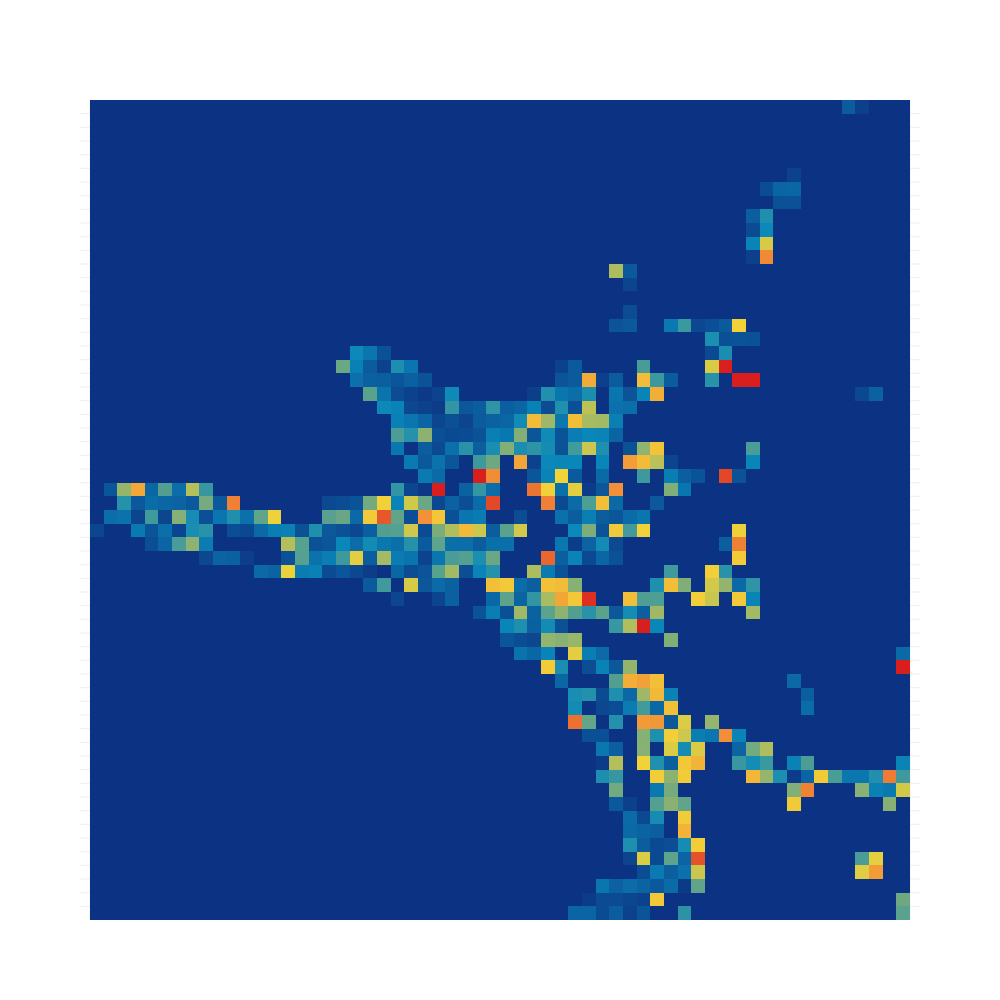
\includegraphics[width=0.5\linewidth]{img/03_empirical_drift.png}}
  \subfloat[Smoothened field]{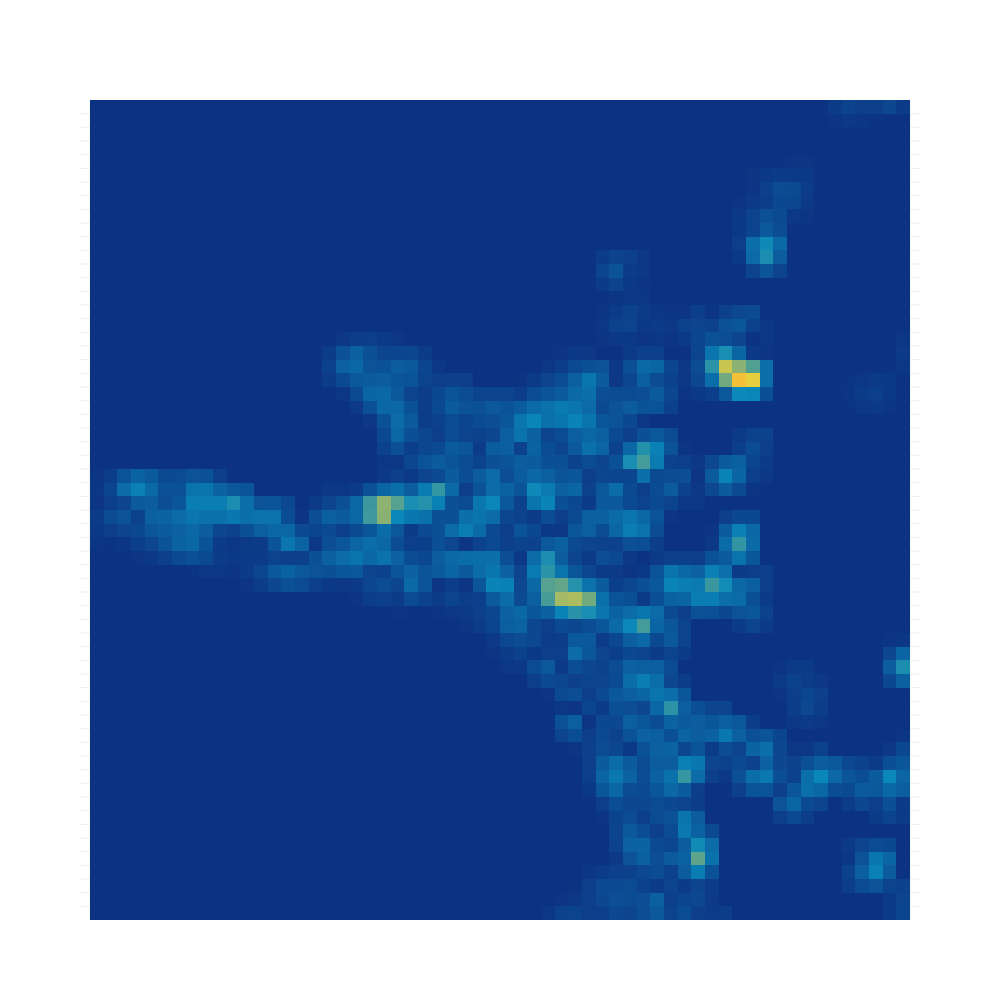
\includegraphics[width=0.5\linewidth]{img/03_smooth_drift.png}}
  \caption{The modulus of the drift field before (a) and after (b) the application of the filter in a subregion of the domain.}
\end{figure}

The simulated trajectories are obtained by forward Euler's scheme
\begin{equation}
\bm{x}_{n+1} = \bm{x}_n + \bm{\tilde{a}}(\bm{x_n})\Delta t
\end{equation}
where $\bm{\tilde{a}}$ is the filtered and smoothed drift field.

We can choose a quite large simulation timestep as the dynamics is deterministic. The coarse grained field has a spatial resolution of $l$ corresponding to the side of the square bins, so we are interested in having, on average, a step size close to the order of $l$. I chose
\begin{equation}
\Delta t = \frac{1}{10} \frac{l}{\langle|\bm{\tilde{a}}|\rangle}
\end{equation}
where $\langle\cdot\rangle$ denotes the mean over the whole spatial domain of $\bm{\tilde{a}}$.

The results of the simulation are shown in figure \ref{fig:simulation}. An example of the attractors localized is visible in figure \ref{fig:attractors}.


\begin{figure}[htb]
  \subfloat[t = 5]{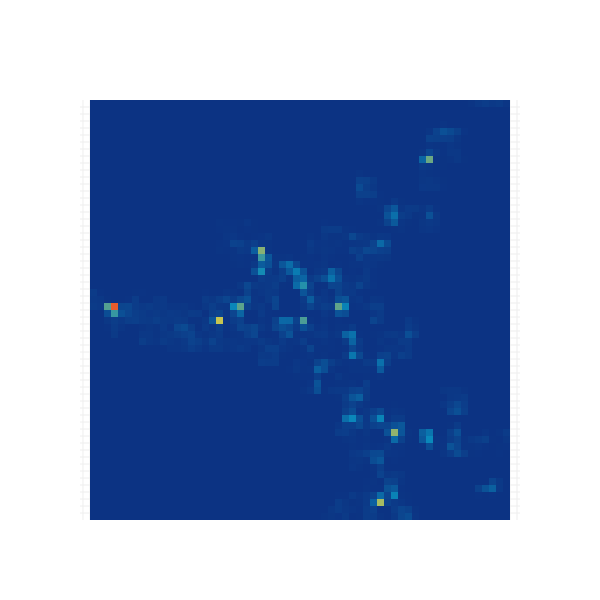
\includegraphics[width=0.33\linewidth]{img/03_005_sim.png}}
  \subfloat[t = 10]{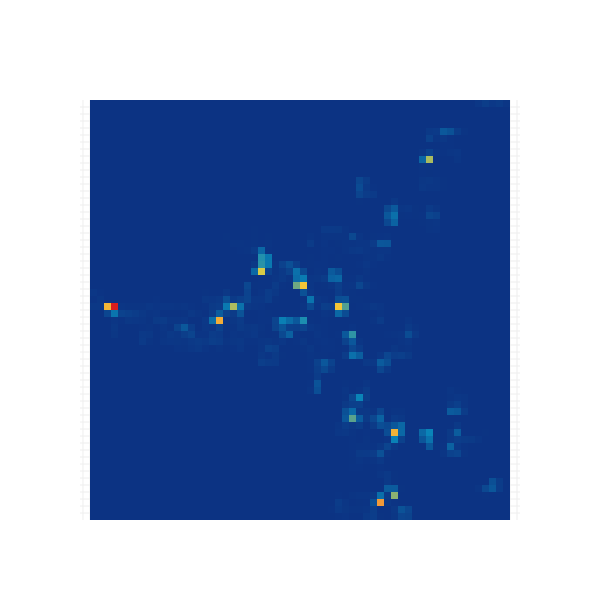
\includegraphics[width=0.33\linewidth]{img/03_010_sim.png}}
  \subfloat[t = 500]{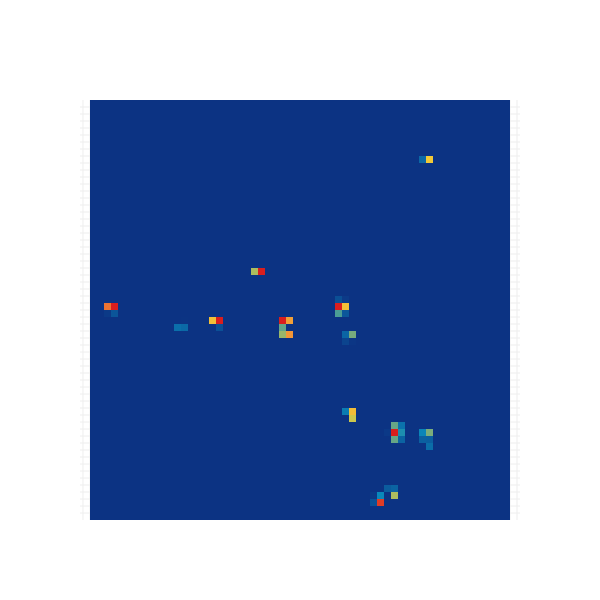
\includegraphics[width=0.33\linewidth]{img/03_500_sim.png}}
  \caption{The density of particles evolution during the simulation in a subregion of the total domain. After 500 steps the particles appear trapped into the attractors.}
  \label{fig:simulation}
\end{figure}


\begin{figure}[htb]
  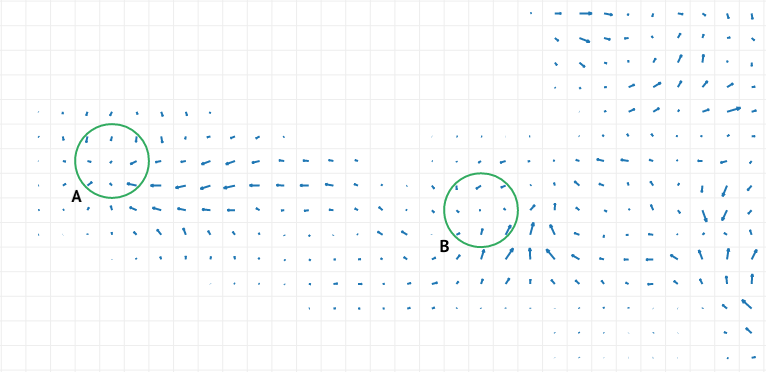
\includegraphics[width=\linewidth]{img/03_attractors.png}
  \caption{Two examples of attractors localized via the numerical simulation. Their weights are $W_A = 7,03 \times 10^{-5}$ and $W_B = 2,06 \times 10^{-5}$.}
  \label{fig:attractors}
\end{figure}


\section{Channels}

\subsection{Channels as potential valleys}

Characterizing the channels is a more challenging task. In fact, if attractors are features well localized in space, channels on the contrary are structures which spread on a moderately large region of space. It becomes difficult to relate them to local features of the field as we did with attractors.

Because of the non-locality, analyzing directly the drift field seems complicated. Instead, I assumed again the field to be generated taking the gradient of a scalar potential $U$ (eq. \ref{eq:conservative}). Putting aside the drift field $\bm{a}$ for one moment, we can try to find a description of channels with respect to the potential $U$.

From this viewpoint, channels are valleys in the surface defined by the potential function, i.e. they are one-dimension local minima of $U$. Features of this type for a two-dimensional scalar function are well known in computer vision, where ridge (and valley) detection is used to identify the main axis of long objects. Reconstructing the potential function would allow to translate the problem from channel detection to ridge detection, thus inheriting from computer vision an already developed toolset for studying these structures.

\subsection{Building the potential}

The empirical field $\bm{a}$ is defined on the square lattice of side $l$ formed by the centres of each bin $S_l$. I indicate with $\bm{a}_{i,j}$ the estimated value of the drift field at row $i$ and column $j$ of the lattice. I similarly define $U$ on a square lattice formed by the middle points between the bin centres. In this way, eq. \ref{eq:conservative} can be represented by the discrete partial derivatives
\begin{align}
a^x_{i,j} &= - \frac{U_{i+1,j} - U_{i,j}}{l} \\[10pt]
a^y_{i,j} &= - \frac{U_{i,j+1} - U_{i,j}}{l}
\end{align}

Fixing an initial condition as $U_{k,m} = c$, it is possible to recover the values of $U$ on the whole lattice iteratively using
\begin{align}
U_{i+1,j} = -a^x_{i,j}l + U_{i,j} \\[10pt]
U_{i,j+1} = -a^y_{i,j}l + U_{i,j}
\end{align}

For this method to work effectively we need a cluster of connected sites where the field $\bm{a}$ is defined and one initial condition for $U$ is fixed. This is not the case for the rough estimated field, since it is full of holes and discontinuities that would prevent us from building a smooth potential. Note also that for isolated bins we have no possibility of reconstructing the potential. To overcome this problems I used the same approach described in section~\ref{sec:attractors} to smoothen the empirical field by first eliminating isolated bins and then convolving with the kernel defined in eq.~\ref{eq:kernel}.

Since the drift field is not perfectly conservative, integrating in one direction or another may produce different potential values for the same lattice site. To minimize these differences I built the potential exploring the neighbouring sites using a breadth first search algorithm and taking the mean when multiple choices of the integration direction were available.



\clearpage

\begin{thebibliography}{9}
\bibitem{hoze2012}
Hoz\'e N, Nair D, Hosy E, Sieben C, Manley S, et al. 2012. \textit{Heterogeneity of receptor trafficking and molecular interactions revealed by superresolution analysis of live cell imaging.} PNAS 109:17052–57

\bibitem{hoze2014}
Hoz\'e N, Holcman D. 2014. \textit{Residence times of receptors in dendritic spines analyzed by stochastic simulations in empirical domains.} Biophys. J. 107:3008–17

\bibitem{schuss}
Schuss, Z. 2010. \textit{Theory and applications of stochastic processes: an analytical approach.} Springer, New York.

\end{thebibliography}



\end{document}
